% !TeX spellcheck = en_US
\documentclass[12pt,fleqn]{article}


\usepackage[english]{babel}

\usepackage{texfiles/SpeedyGonzales}
\usepackage{texfiles/MediocreMike}
\usepackage{verbatim} 













\title{Bayesian Optimization for Hyperparameter Tuning in the Fully Connected Layers of VGG16}
\author{Søren Winkel Holm\and Oskar Wiese\and Anders Henriksen\and Anne Agathe Pedersen}
\date{\today}

\fancypagestyle{plain}
{
	\fancyhf{}
	\rfoot{Page \thepage{} of  \pageref{LastPage}}
	\renewcommand{\headrulewidth}{0pt}
}
%\pagestyle{fancy}
%\fancyhf{}
%\lhead{Lala}
%\chead{}
%\rhead{}
%\rfoot{Page \thepage{} of \pageref{LastPage}}

\graphicspath{{imgs/}}
\usepackage{float}
\usepackage[caption = false]{subfig}
%\linespread{1.15}

%TODO: \numberwithin{equation}{section}
%TODO: \numberwithin{footnote}{section}
%TODO: \numberwithin{figure}{section}
%TODO: \numberwithin{table}{section}

\begin{document}






\maketitle

%\tableofcontents
%\thispagestyle{fancy}
%\tableofcontents

\begin{abstract}

Optimization of neural network hyperparameters is a costly process usually pervaded by uncertainty. 
This report combines Bayesian optimization with Gaussian processes to find optimal hyperparameters for the VGG16 image classification network when training on the CIFAR10 dataset. 
%What is our big idea? What research, analysis, and experiment did we do?
%What is the answer to our questions?
%What are the implications of our findings?

\end{abstract}


\section{Introduction} 
Humans are slow and faulty. This means that work costs heaps of money and mistakes happen often. To help mitigate this, machine learning can learn the task at hand in order to optimize the performance at a much lower cost. While effective for many applications, machine learning has one glaring issue that requires skill and tonnes of computing power to overcome; hyperparameter optimization. Optimizing the hyperparameters usually devolves into random guessing, though new methods are on the rise like Bayesian optimization, which greatly reduces the effort involved in finding the parameters with use of an acquisition function and probabilistic model.

In this paper, Bayesian optimization with Gaussian processes as probabilistic model and expected improvement, upper confidence bound and probability of improvement as acquisition function will be used to find the hyperparameters of the VGG16 classifier network when training to classify on the 10 classes of the CIFAR10 dataset, optimizing for the validation accuracy.


\section{Methods}
Gaussian process and Bayesian optimization...

Three different aquisition functions + random...

\subsection*{Gaussian Process}


\subsection*{Acquisition Functions}
In the following section three different acquisition functions will be presented. All of these acquisition functions are implemented by using the GPyOpt library. \newline
\noindent\\
\textbf{Probability of Improvement} \\
Probability of improvement evaluates \textit{f}, the objective function, at the point most likely to improve the minimum value. In this project, the objective function returns the negative validation accuracy. Probability of improvement then evaluates at the point most likely to obtain a higher accuracy, since the the function is given the negative accuracy. Mathematically PI can be expressed as,
\begin{equation*}
	\text{PI}(\mathbf{x}) = \text{P}(f(\mathbf{x}) \geq f(\mathbf{x}^+) + \xi) 
	= \Phi\biggl(\frac{\mu(\mathbf{x}) - f(\mathbf{x}^+) - \xi}{\sigma(\mathbf{x})}\biggr)
\end{equation*}
\noindent
where $\xi$ is a hyperparameter which can be set by the user. The hyperparameter is a trade off between exploration and exploitation. $\Phi$ is the cumulative distribution function of the Gaussian distribution.
\newline \\
\textbf{Expected Improvement} \newline 
The expectorated improvement tries to quantify the improvement instead of the probability of improving as Probability of Improvement does. It is possible to quantify the average value of improvement if we sample the objective function at $ x $. The acquisition function then computes the expected value of the improvement function at a certain x. Mathematically EI can be expressed as, 
\begin{equation*}
\mathrm{EI}(\mathbf{x})=\left\{\begin{array}{ll}
\left(\mu(\mathbf{x})-f\left(\mathbf{x}^{+}\right)\right) \Phi(Z)+\sigma(\mathbf{x}) \phi(Z) & \text { if } \sigma(\mathbf{x})>0 \\
0 & \text { if } \sigma(\mathbf{x})<0
\end{array}\right. 
\end{equation*}
Here the variable $ Z = \frac{\mu(\mathbf{x}) - f(\mathbf{x}^+) - \xi }{\sigma(\mathbf{x})} $ \newline 
\\
\textbf{Gaussian Process Upper Confidence Bound} \newline
The idea behind the GP-UCB is to directly use the mean and variance from the Gaussian distribution. These two parameters are used as the exploration / exploitation trade off. The function UCB (Ubber Confidence Bound) can be formulated as the following, 
\begin{equation*}
UCB(x) = \mu(x) + \kappa \sigma(x)
\end{equation*}
\noindent
Where $ \kappa $ is a user defined variable used to control the trade off between exploration and exploitation. \newline

\subsection*{Grid Search}

\section{Results}

\begin{table}[H]\label{resultater}
	\begin{tabular}{|l|l|l|l|l|}
		\hline
		Optimal parameters for & Hidden units & Dropout probability & Activation & Validation Accuracy \\ \hline
		BO: EI  & 2540         & 16\pro              & Tanh             &    62.8\pro       \\ \hline
		BO: MPI & 2403         & 61\pro             & Sigmoid             & 64.7\pro            \\ \hline
		BO: UCB & 1150         & 53\pro              & Sigmoid             & 64.6\pro           \\ \hline
		Grid Search & 2000         & 66\pro              & Sigmoid             & 64.9\pro          \\ \hline
	\end{tabular}
\caption{Bayesian optimization has been performed with three different acquisition functions. The optimal hyper-parameters are presented in the table as well as the accuracy of the VGG16 with these specific hyper-parameters. At the bottom of the table a Grid Searching scheme has been implemented to compete against the baysian classifier. All of the results can be seen in the Appendix. }
\end{table}
\begin{figure}[H]
	\centering

	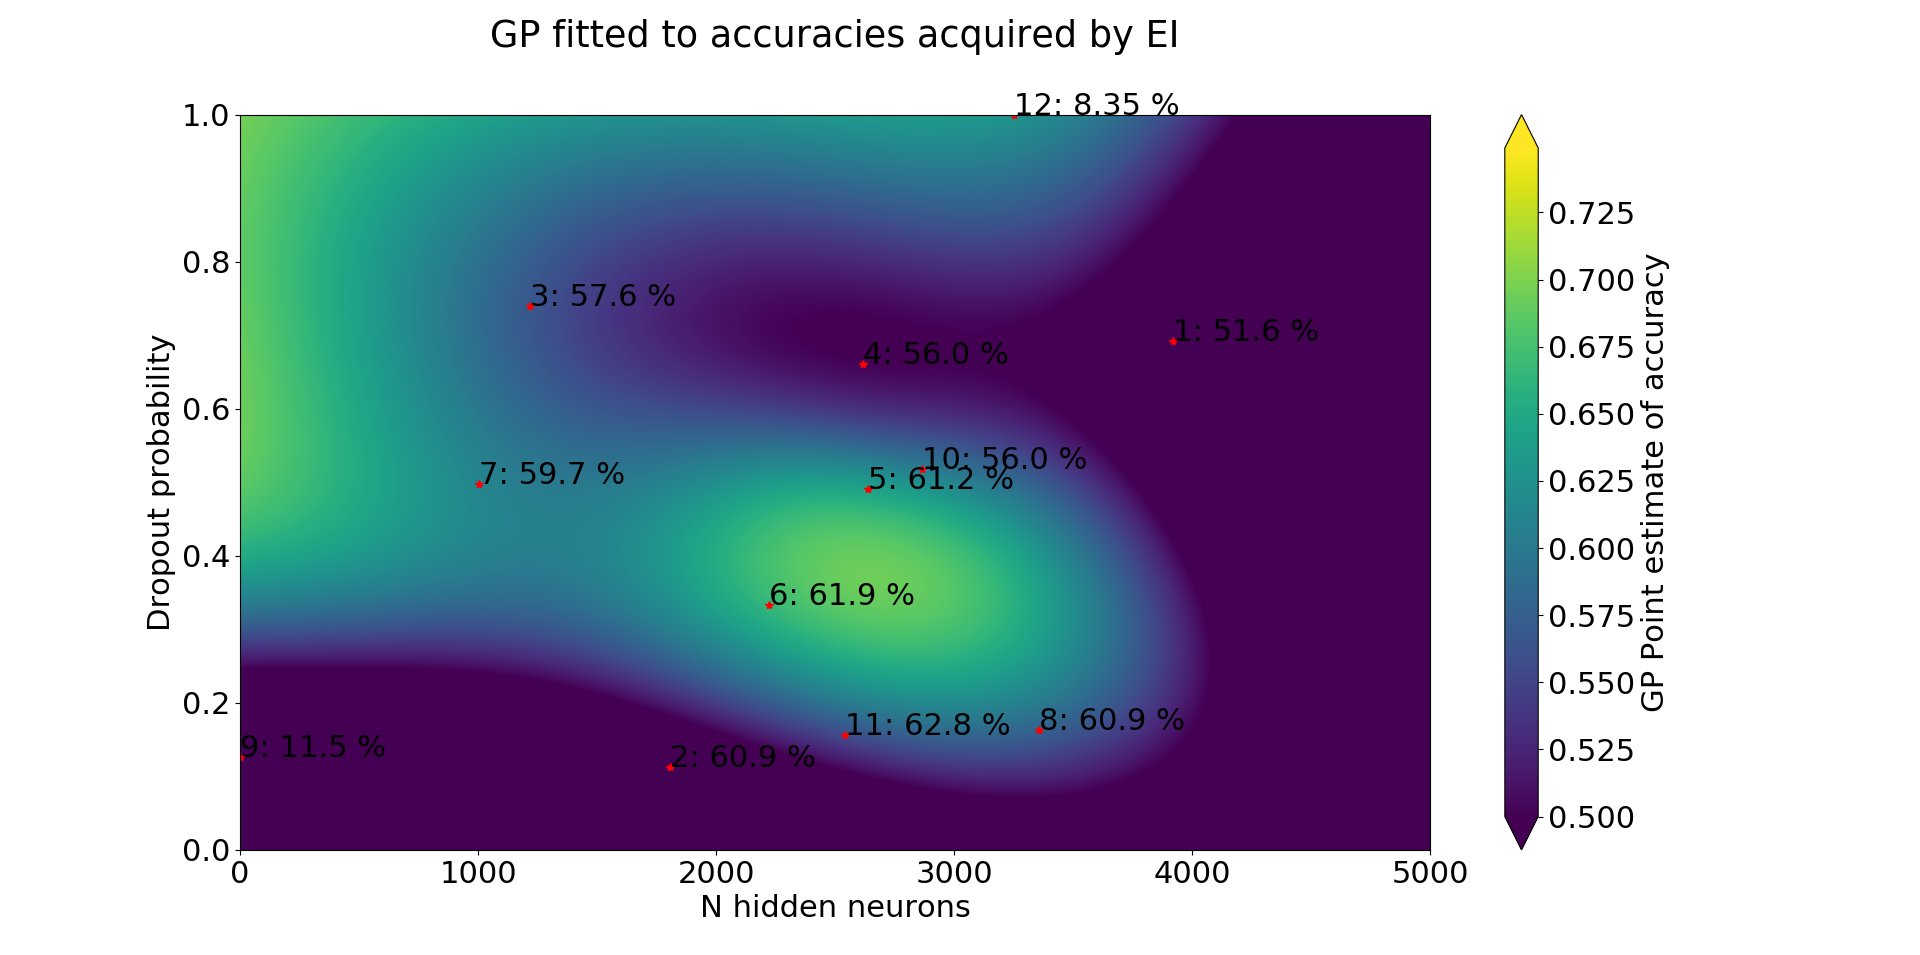
\includegraphics[width=\textwidth]{EIGP}	

\caption{The Gaussian process fitted to the twelve accuracy points acquired by the expected improvement function. It can be seen that bla bla bla. Visualizations for other acquisition functions in appendix.}
\end{figure}
\begin{comment}
	Results of using baysian optimization with acquisition MPI: \\
	${hidden units: 3500, p: 0.4423657706097197, activation func: Sigmoid(), validation loss: 0.6415}$
	${hidden units: 600, p: 0.05357242679336405, activation func: ReLU(), validation loss: 0.6135}$
	${hidden units: 800, p: 0.024286531237800668, activation func: Sigmoid(), validation loss: 0.624}$
	${hidden units: 900, p: 0.5359999678433617, activation func: Tanh(), validation loss: 0.621}$
	${hidden units: 900, p: 0.6064720199905345, activation func: Tanh(), validation loss: 0.6215}$
	${hidden units: 3500, p: 0.28760052084452836, activation func: Sigmoid(), validation loss: 0.639}$
	${hidden units: 3500, p: 0.4812338027466384, activation func: Sigmoid(), validation loss: 0.649}$
	${hidden units: 3500, p: 0.598166666688632, activation func: Sigmoid(), validation loss: 0.654}$
	${hidden units: 3500, p: 0.7073019913319729, activation func: Sigmoid(), validation loss: 0.635}$
	${hidden units: 3500, p: 0.6366823572272423, activation func: Sigmoid(), validation loss: 0.6455}$
	${hidden units: 3500, p: 0.7208836418636946, activation func: Sigmoid(), validation loss: 0.6425}$
	${hidden units: 3500, p: 0.8135979227010048, activation func: Sigmoid(), validation loss: 0.6045}$
	${hidden units: 3500, p: 0.5757959667629431, activation func: Sigmoid(), validation loss: 0.6535}$
	${hidden units: 3500, p: 0.5577435983137187, activation func: Sigmoid(), validation loss: 0.6535}$
	${hidden units: 3500, p: 0.4119006857770867, activation func: Sigmoid(), validation loss: 0.6295000000000001}$
	$bedste:  [3.5000000e+03 2.8204313e-01 3.0000000e+00]$
	
	Results of using baysian optimization with acquisition EI: \\
	${hidden units: 2900, p: 0.2120309217292945, activation func: Sigmoid(), validation loss: 0.6535}$
	${hidden units: 1300, p: 0.16575828954515115, activation func: ReLU(), validation loss: 0.6465}$
	${hidden units: 200, p: 0.9318047460286568, activation func: Tanh(), validation loss: 0.335}$
	${hidden units: 2200, p: 0.7223805260392725, activation func: ReLU6(), validation loss: 0.4905}$
	${hidden units: 1200, p: 0.05956534512526279, activation func: ReLU6(), validation loss: 0.6355000000000001}$
	${hidden units: 2900, p: 1.0, activation func: Sigmoid(), validation loss: 0.135}$
	${hidden units: 2900, p: 0.18851940843012052, activation func: Sigmoid(), validation loss: 0.6545}$
	${hidden units: 1300, p: 0.5317365663075784, activation func: Sigmoid(), validation loss: 0.665}$
	${hidden units: 1300, p: 1.0, activation func: Sigmoid(), validation loss: 0.099}$
	${hidden units: 1300, p: 0.37484134186025747, activation func: Sigmoid(), validation loss: 0.6635}$
	${hidden units: 1200, p: 0.43302270846068275, activation func: ReLU6(), validation loss: 0.6145}$
	${hidden units: 1200, p: 0.9814408341697629, activation func: ReLU6(), validation loss: 0.097}$
	${hidden units: 1300, p: 0.36590712967937133, activation func: Sigmoid(), validation loss: 0.657}$
	${hidden units: 1300, p: 0, activation func: Sigmoid(), validation loss: 0.6275000000000001}$
	${hidden units: 1300, p: 0.16460856311701932, activation func: ReLU(), validation loss: 0.6395000000000001}$
	$bedste:  [1.30000000e+03 5.31736566e-01 3.00000000e+00]$
	
	Results of using baysian optimization with acquisition LCB: \\
	${hidden units: 3300, p: 0.20745359704991084, activation func: ReLU(), validation loss: 0.619}$
	${hidden units: 2900, p: 0.48178037973857923, activation func: Sigmoid(), validation loss: 0.6355}$
	${hidden units: 1700, p: 0.37725127529617486, activation func: ReLU6(), validation loss: 0.5955}$
	${hidden units: 3400, p: 0.5452219321218295, activation func: Sigmoid(), validation loss: 0.6275}$
	${hidden units: 1800, p: 0.47970862684081317, activation func: ReLU(), validation loss: 0.613}$
	${hidden units: 2900, p: 0.4817801130255398, activation func: Sigmoid(), validation loss: 0.634}$
	${hidden units: 2900, p: 0.4891192307830994, activation func: Sigmoid(), validation loss: 0.642}$
	${hidden units: 2900, p: 0.4947118739255611, activation func: Sigmoid(), validation loss: 0.6365}$
		${hidden units: 2900, p: 0.5834934845352279, activation func: Sigmoid(), validation loss: 0.651}$
	${hidden units: 2900, p: 0.6168247073529851, activation func: Sigmoid(), validation loss: 0.6365}$
	${hidden units: 2900, p: 1, activation func: Sigmoid(), validation loss: 0.0965}$
	${hidden units: 2900, p: 0.5604663271240786, activation func: Sigmoid(), validation loss: 0.635}$
	${hidden units: 2900, p: 0.5094736622953687, activation func: Sigmoid(), validation loss: 0.638}$
	${hidden units: 2900, p: 0.5849237064289087, activation func: Sigmoid(), validation loss: 0.629}$
	${hidden units: 2900, p: 0.5765931111057664, activation func: Sigmoid(), validation loss: 0.6265}$
	$bedste:  [2.90000000e+03 5.83493485e-01 3.00000000e+00]$	
\end{comment}

\begin{comment}
	{'hidden_units': 100, 'p': 0.33, 'activation_func': Sigmoid()}
	0.6345000000000001
	
	{'hidden_units': 100, 'p': 0.33, 'activation_func': Sigmoid()}
	0.6405
	
	{'hidden_units': 100, 'p': 0.66, 'activation_func': ReLU()}
	0.515
	
	{'hidden_units': 100, 'p': 0.66, 'activation_func': Sigmoid()}
	0.561
	
	{'hidden_units': 2000, 'p': 0.33, 'activation_func': Tanh()}
	0.513
	
	{'hidden_units': 2000, 'p': 0.33, 'activation_func': ReLU()}
	0.649
	
	{'hidden_units': 2000, 'p': 0.66, 'activation_func': Sigmoid()}
	0.6525
	
	{'hidden_units': 2000, 'p': 0.66, 'activation_func': ReLU6()}
	0.5685
	
	{'hidden_units': 4000, 'p': 0.33, 'activation_func': Tanh()}
	0.5595
	
	{'hidden_units': 4000, 'p': 0.33, 'activation_func': ReLU6()}
	0.5345
	
	{'hidden_units': 4000, 'p': 0.66, 'activation_func': ReLU6()}
	0.5015000000000001
	
	{'hidden_units': 4000, 'p': 0.66, 'activation_func': Tanh()}
	0.505
	
\end{comment}

\section{Discussion}
%In this section you interpret your findings and describe why they are important and how they fit in with
%other research. You can also mention ways your study could have been improved and future areas of
%research.
% What might the answer imply, and what does it matter?
% How does it fit in with what other researchers have found?
% What are the perspectives for future research? 

From the table seen in results \ref{resultater}, Bayesian optimization has proposed hyper-parameters that makes the accuracy higher than the hyper-parameters found using GridSearch. However, the difference in accuracies between the model proposed by Bayesian optimization and GridSearch are $ \Delta p = 0.011$. Too see if there is an actual significant difference between the accuracy of the models a McNemar test can be performed. This is beyond the scope of this project and will be left for future work. In reality a McNemar test would probably show that there is no significant difference between the accuracy of the two models. Hence, this shows that a random search grid and Bayseian Optimization finds hyper-parameters for VGG16 that are equally good.
\\\\
The results discovered in this project prove that Bayesian Optimization can indeed be used for hyper-parameter tuning and is faster than Grid Search. The advantage of Bayesian Optimization is the fact, that it does not explore parts of the parameter space because it believes these areas does not contain parameters that maximizes the accuracy of VGG16. This fact limits the amount of time used for training the model. 

\section{References}
\url{https://gpyopt.readthedocs.io/en/latest/index.html}
\section{Appendix}
\begin{figure}[H]

		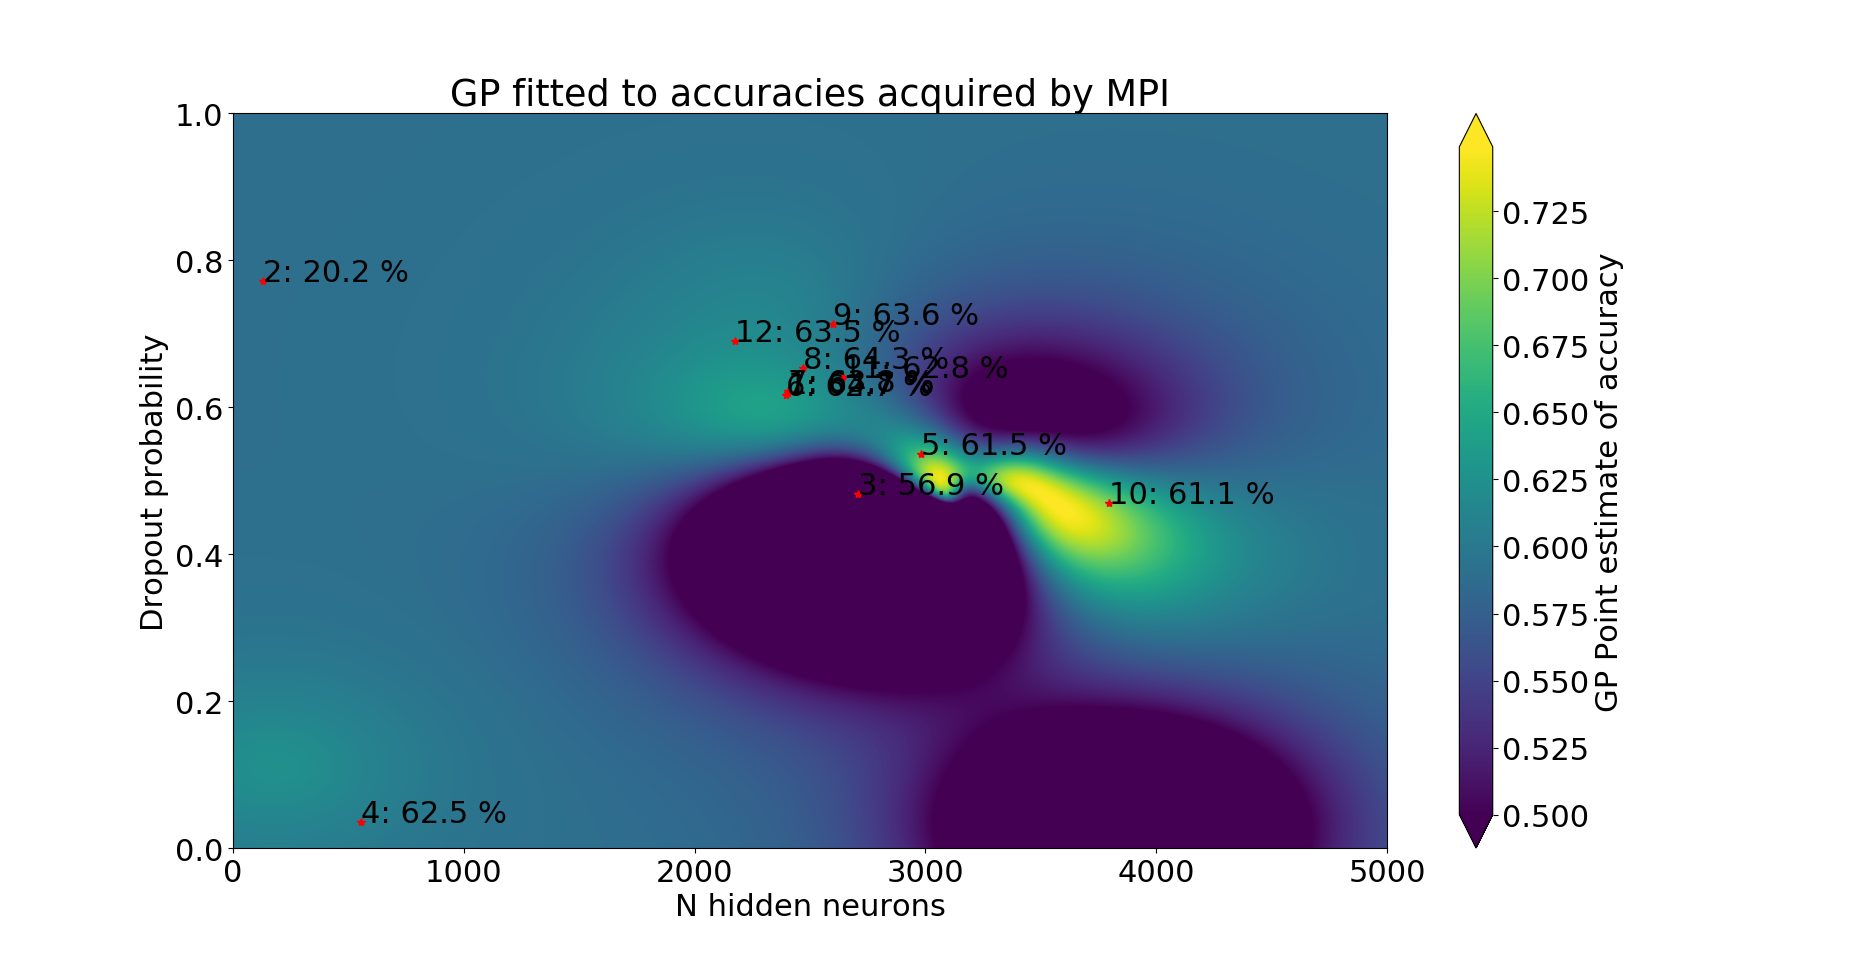
\includegraphics[width=\textwidth]{MPIGP}	
\end{figure}
\begin{figure}[H]
		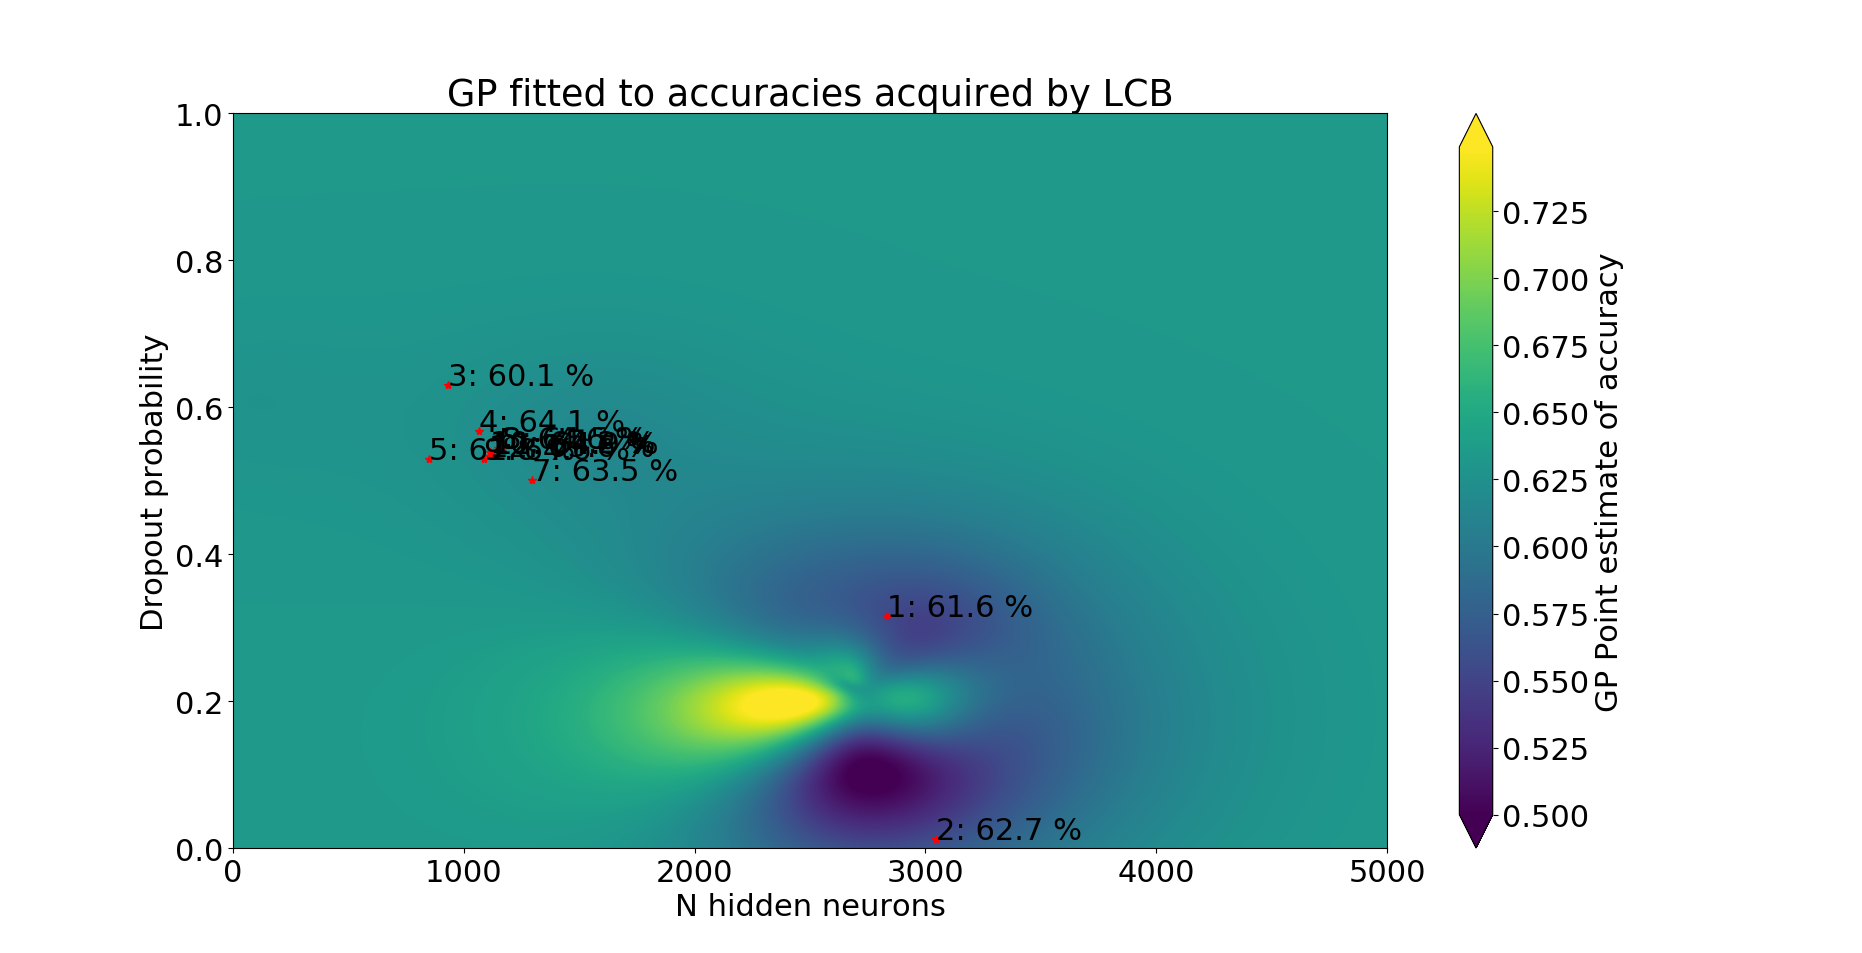
\includegraphics[width=\textwidth]{LCBGP}	

\end{figure}
EI
\begin{table}[H]
	\begin{tabular}{|l|l|l|l|l|}
		\hline
		Iteration & Hidden units & Dropout probability & Activation function & Accuracy \\ \hline
		1 & 3917 & 0.6923 & 1 & 0.5165 \\ \hline 

		2 & 1805 & 0.1127 & 0 & 0.609 \\ \hline 

		3 & 1217 & 0.7398 & 2 & 0.5765 \\ \hline 

		4 & 2618 & 0.6605 & 1 & 0.5605 \\ \hline 

		5 & 2639 & 0.491 & 0 & 0.6115 \\ \hline 

		6 & 2220 & 0.3325 & 0 & 0.6185 \\ \hline 

		7 & 1002 & 0.4978 & 0 & 0.5965 \\ \hline 

		8 & 3354 & 0.1637 & 0 & 0.609 \\ \hline 

		9 & 1 & 0.1262 & 1 & 0.1145 \\ \hline 

		10 & 2863 & 0.5179 & 0 & 0.5595 \\ \hline 

		11 & 2540 & 0.1569 & 0 & 0.6275000000000001 \\ \hline 

		12 & 3251 & 1.0 & 2 & 0.0835 \\ \hline 

	\end{tabular}
\end{table}
MPI

\begin{table}[H]
	\begin{tabular}{|l|l|l|l|l|}
		\hline
		Iteration & Hidden units & Dropout probability & Activation function & Accuracy \\ \hline
1 & 2403 & 0.6196 & 3 & 0.647 \\ \hline 

2 & 130 & 0.7724 & 1 & 0.202 \\ \hline 

3 & 2706 & 0.4818 & 0 & 0.5685 \\ \hline 

4 & 554 & 0.03571 & 2 & 0.6245 \\ \hline 

5 & 2983 & 0.5369 & 1 & 0.6145 \\ \hline 

6 & 2397 & 0.6166 & 3 & 0.6275 \\ \hline 

7 & 2407 & 0.6219 & 3 & 0.6385 \\ \hline 

8 & 2471 & 0.6537 & 3 & 0.6435 \\ \hline 

9 & 2601 & 0.7138 & 3 & 0.636 \\ \hline 

10 & 3794 & 0.4693 & 1 & 0.611 \\ \hline 

11 & 2641 & 0.6416 & 3 & 0.6285 \\ \hline 

12 & 2176 & 0.69 & 3 & 0.6355 \\ \hline 

	\end{tabular}
\end{table}



LCB
\begin{table}[H]
	\begin{tabular}{|l|l|l|l|l|}
		\hline
		Iteration & Hidden units & Dropout probability & Activation function & Accuracy \\ \hline
		1 & 2835 & 0.316 & 2 & 0.616 \\ \hline 
		2 & 3046 & 0.01182 & 3 & 0.627 \\ \hline 
		3 & 934 & 0.6308 & 0 & 0.6005 \\ \hline 
		4 & 1068 & 0.5681 & 3 & 0.641 \\ \hline 
		5 & 848 & 0.5295 & 1 & 0.6175 \\ \hline 
		6 & 1150 & 0.5441 & 3 & 0.646 \\ \hline 
		7 & 1297 & 0.5009 & 3 & 0.635 \\ \hline 
		8 & 1165 & 0.5443 & 3 & 0.6455 \\ \hline 
		9 & 1089 & 0.5296 & 3 & 0.646 \\ \hline 
		10 & 1115 & 0.5386 & 3 & 0.6425 \\ \hline 
		11 & 1127 & 0.5375 & 3 & 0.649 \\ \hline 
		12 & 1112 & 0.5333 & 3 & 0.636 \\ \hline 
	\end{tabular}
\end{table}
 
 
grid search
\begin{table}[H]
	\begin{tabular}{|l|l|l|l|l|}
		\hline
		Iteration & Hidden units & Dropout probability & Activation function & Validation loss \\ \hline
		1         & 100          & 0.33                & Sigmoid             & 0.6345          \\ \hline
		2         & 100          & 0.33                & Sigmoid             & 0.6405          \\ \hline
		3         & 100          & 0.66                & ReLU                & 0.5150          \\ \hline
		4         & 100          & 0.66                & Sigmoid             & 0.5610          \\ \hline
		5         & 2000         & 0.33                & Tanh                & 0.513           \\ \hline
		6         & 2000         & 0.33                & ReLU                & 0.649           \\ \hline
		7         & 2000         & 0.66                & Sigmoid             & 0.6525          \\ \hline
		8         & 2000         & 0.66                & ReLU6               & 0.5685          \\ \hline
		9         & 4000         & 0.33                & Tanh                & 0.5595          \\ \hline
		10        & 4000         & 0.33                & ReLU6               & 0.5345          \\ \hline
		11        & 4000         & 0.66                & ReLU6               & 0.5015          \\ \hline
		12        & 4000         & 0.66                & Tanh                & 0.5050          \\ \hline
	\end{tabular}
\end{table}

\end{document}

















